\documentclass[a4paper, 11pt, twoside]{article}

\usepackage[brazilian]{babel}
\usepackage[utf8]{inputenc}
\usepackage[T1]{fontenc}
\usepackage{fixltx2e}
\usepackage{amsmath}
\usepackage{amssymb}
\usepackage{graphicx}
\usepackage{float}
\usepackage{a4wide}
\usepackage{multicol}
\usepackage{xcolor}
\usepackage{makeidx}
\usepackage{hyperref}
\usepackage{textcomp}

\setcounter{tocdepth}{2}

\graphicspath{ {./fig/} }

\newcommand{\HRule}{\rule{\linewidth}{0.5mm}}
\newcommand{\pdobject}[1]{\begin{center}\fbox{\texttt{#1}}\end{center}}

\begin{document}

\hypersetup{backref,pdfpagemode=FullScreen,colorlinks=true}

\begin{titlepage}

\begin{center}
% Upper part of the page

%\includegraphics[width=0.15\textwidth]{./usp.jpg}\\[1 cm]

\textsc{\LARGE Universidade de São Paulo}\\
\textsc{\Large Pró-Reitoria de Graduação}\\
\textsc{\Large Curso de Ciências Moleculares}\\[1.5cm]
\textsc{\Large Relatório Final de Iniciação Científica}\\[0.5cm]

% Title
\HRule \\[0.4cm]
{ \LARGE \bfseries Interfaces entre o Usuário e Sistemas Musicais Multiagentes}\\[0.4cm]

\HRule \\[1.5cm]

% Author and supervisor
\begin{minipage}{0.4\textwidth}
\begin{flushleft} \normalsize
\emph{Autor:}\\
Pedro H. R. \textsc{Bruel} \\
\vspace{0.3cm}
\emph{Email:}\\
pedro.bruel@gmail.com \\
\vspace{0.3cm}
\emph{Telefone: 97587-2511}\\
\vspace{0.3cm}
\emph{Turma: 20}\\
\end{flushleft}
\end{minipage}
\begin{minipage}{0.5\textwidth}
\begin{flushright} \normalsize
\emph{Orientador:} \\
Prof Dr Marcelo \textsc{Queiroz} \\
\vspace{0.3cm}
\emph{Email:}\\
mqz@ime.usp.br \\
\vspace{0.3cm}
\emph{Unidade: }\\
Instituto de Matemática e Estatística \\
\vspace{0.3cm}
\emph{Departamento: }\\
Ciência da Computação\\
\end{flushright}
\end{minipage}
\vfill
% Bottom of the page
{\large 2º Semestre de 2013}

\end{center}

\end{titlepage}


\tableofcontents
\newpage

\begin{abstract}
\line(1,0){350}

A adaptabilidade em tempo real e o potencial de modelagem de sistemas complexos
são características de Sistemas Multiagentes, que têm variadas aplicações no 
contexto musical. A ferramenta de criação musical e linguagem de programação 
Pure Data (Pd) é tradicionalmente utilizada por músicos em performances 
musicais. Este projeto produziu uma integração do arcabouço para Sistemas
Multiagentes Musicais Ensemble - implementado pelo Grupo de Computação Musical 
do IME/USP - com a libpd, uma infraestrutura do tipo API para Pure Data. 
A integração procura facilitar a utilização do arcabouço por usuários 
não programadores. A interface é uma extensão do Arcabouço Ensemble,
e permite desenvolver aplicações do Arcabouço através do ambiente gráfico
do Pure Data.

\line(1,0){350}
\end{abstract}

\begin{multicols}{2}

\section{Introdução}

Este relatório descreve e detalha as atividades desenvolvidas no período de 
Fevereiro a Julho de 2014, sumarizadas a seguir.

O aluno apresentou um seminário sobre o trabalho desenvolvido na elaboração da 
interface entre a linguagem de programação Pure Data e o Arcabouço Ensemble, 
no ciclo aberto de seminários do Grupo de Computação Musical.

Elaborou-se um protocolo de comunicação entre o Arcabouço Ensemble e o
Pure Data, permitindo a comunicação entre \textit{patches} e o Arcabouço.

A interface de comunicação básica implementada no semestre passado foi
largamente estendida durante este semestre, permitindo a definição de
Agentes Musicais, seus Raciocínios e Componentes e até aplicações
completas do Arcabouço Ensemble através de \textit{patches} Pure Data.

Submetemos um artigo para a Conferência Conjunta ICMC/SMC 2014~\cite{},
detalhando o protocolo e a interface desenvolvidos. O artigo foi aceito
para publicação e apresentação oral na Conferência.

As próximas seções apresentam o detalhamento destas atividades e 
contextualizam o trabalho realizado, discutindo a linguagem Pure Data
e o Arcabouço Ensemble. O artigo publicado na Conferência Conjunta ICMC/SMC
2014 segue em anexo ao relatório.

\section{Sistemas Multiagentes}

Um Sistema Multiagentes é composto~\cite{wooldridgeART, jennings99} de um 
Ambiente virtual e Agentes computacionais. A interação entre os Agentes 
contidos no ambiente é influenciada pelos parâmetros e características desse 
Ambiente. As seções seguintes detalharão as propriedades de cada componente.

\subsection{Agente}

Entidade computacional com interfaces e características bem definidas, 
orientada e instrumentalizada para a solução de problemas computacionais em 
geral~\cite{jennings99}. Para o propósito deste projeto, significa uma 
estrutura que aprensenta as seguintes propriedades~\cite{wooldridgeART}:

\begin{enumerate}
  \item \textbf{Autonomia}: Encapsula estados e é capaz de tomar decisões 
      independentes, baseadas nesses estados;
  \item \textbf{Reatividade}: Está imerso em um Ambiente, é capaz de percebê-lo
      e responder a mudanças;
  \item \textbf{Proatividade}: Pode apresentar ações orientadas por objetivos, 
      tomando iniciativas para alcançá-los;
  \item \textbf{Interação Social}: É capaz de interagir com outros Agentes, ou 
      com usuários, para resolver problemas cooperativamente e atingir 
      seus objetivos.
\end{enumerate}

\subsection{Ambiente}

Contém os Agentes e fornece um meio para as interações entre eles. Pode ser 
implementado como uma simulação do mundo físico, uma interface gráfica com o 
usuário, uma coleção de outros Agentes, e variações e combinações dentre essas 
possibilidades~\cite{wooldridgeART}.

\subsection{Sistemas Multiagentes Musicais}

Um Agente Musical é um Agente especializado em processamento e síntese de 
sinais sonoros e informação musical, e é tipicamente capaz de receber 
informação sonora proveniente do Ambiente ou de outros Agentes através de seus 
Sensores, aplicar algum tipo de Raciocínio sobre essa informação e responder 
de forma adequada através de Atuadores, levando em consideração seus objetivos 
e Base de Conhecimentos - onde ficam armazenadas as informações necessárias ao 
seu funcionamento~\cite{queiroz09, santiago12, leandro11}.

No contexto de um Sistema Multiagentes Musical, um Ambiente é 
composto de uma Representação Física - incluindo definições de parâmetros de 
propagação de som, dimensões espaciais e temporais, e todas as grandezas 
físicas relevantes à representação sonora - e uma Representação Ecológica, que 
define as regras para interação de Agentes, como tempo de vida, reprodução, 
movimentação e demais funções biológicas ou 
comportamentais~\cite{queiroz09, santiago12, leandro11}.

\end{multicols}
\begin{figure}[H]
  \centering
  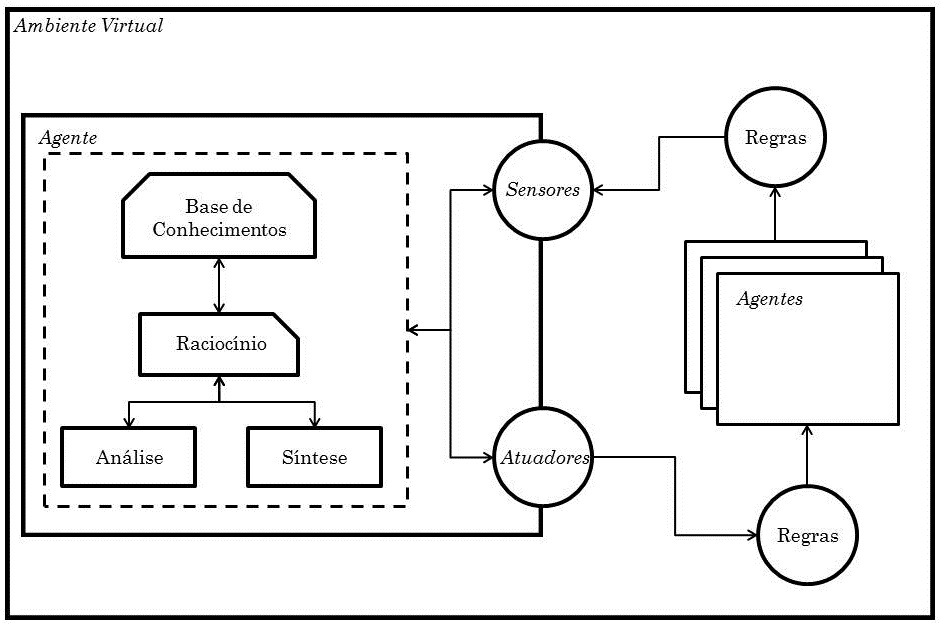
\includegraphics[scale=0.42]{SistMult.jpg}
  \caption{Representação de um Sistema Multiagentes Musical}
  \label{fig:sistmult}

\end{figure}
\begin{multicols}{2}

\section{Sistemas Musicais Multiagentes}

Esta seção apresenta alguns exemplos e aplicações de Sistemas Musicais 
Multiagentes.

\subsection{Aplicações}

Whalley~\cite{whalley05}, aprensenta quatro abordagens para o uso de 
Sistemas Multiagentes no contexto artístico de música e som.

\subsubsection{Simulação}

Agentes simulam estilos pré concebidos, lidando com situações multi-causais em 
tempo real sem entrada humana, interagindo uns com os outros na construção de 
uma estrutura musical. 
  
Em Ramalho \textit{et. al}~\cite{ramalho99}, é apresentado um modelo para um 
baixista virtual numa banda de jazz, numa apresentação ao vivo, sujeito a uma 
platéia e demais músicos. 
  
Em Costalonga \textit{et. al}~\cite{costalonga08}, o modelo é para a interação 
entre as mãos de um guitarrista, que decidem formatos de acordes no braço da 
guitarra.

\subsubsection{Geração} 

Neste tipo de aplicação o foco artístico é o processo de criação, em 
detrimento de um produto com forma pré-determinada. O compositor cria uma 
série de comportamentos~\cite{miranda03} para os Agentes, e a geração de 
conteúdo e até mesmo de uma estrutura musical é resultado da interação 
entre eles.

\subsubsection{Reação à Performance}

Agentes têm seus comportamentos e ações pré-programados para interagir com 
usuários, criando variados tipos de interação em redes com entrada humana.

\subsubsection{Geração e Improvisação}

Permite entrada de improvisações humanas mas, ao invés de uma simples reação 
por parte dos Agentes, ocorrerá geração adaptativa de uma resposta. A resposta 
será então processada pelo improvisador humano, que gerará nova entrada.

\subsection{Exemplos}

Esta seção expõe alguns Sistemas Musicais Multiagentes 
apresentados por diferentes artigos. Os exemplos apresentados procurar 
representar os contextos descritos anteriormente.

\subsubsection{CAMUS e Chaosynth}

O artigo~\cite{miranda2003music} de Eduardo Miranda trata do uso de processos 
computacionais em composição musical, e apresenta o CAMUS e o Chaosynth, dois 
sistemas musicais baseados em autômatos celulares.

\begin{figure}[H]
  \centering
  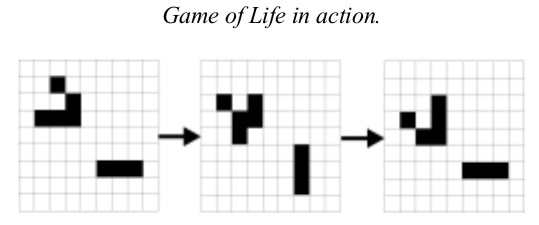
\includegraphics[scale=0.52]{gameoflife1.jpg}
  \caption{Iterações do Tabuleiro do Game of Life~\cite{miranda2003music}}
  \label{fig:game1}

\end{figure}

Uma das partes do CAMUS é uma implementação do Game of Life, um tabuleiro 
bidimensional de autômatos celulares, modelando uma colônia de organismos 
virtuais que seguem regras simples. O tabuleiro é então iterado simulando
interações entre esses organismos, com cada passo representando um estado 
diferente do sistema.

Uma célula preta representa um organismo vivo, e uma branca, um local vago. 
O estado de uma célula numa iteração dependerá das células adjacentes nos 
instantes anteriores. Cada célula representa uma tripla de notas, e cada 
passo do Game of Life gera diferentes triplas.

\begin{figure}[H]
  \centering
  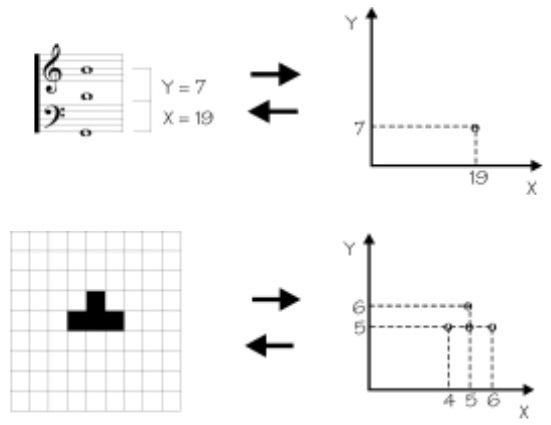
\includegraphics[scale=0.52]{gameoflife2.jpg}
  \caption{Correspondência Musical do Tabuleiro~\cite{miranda2003music}}
  \label{fig:game2}

\end{figure}

O segundo Sistema Musical Multiagente apresentado pelo artigo é o Chaosynth, 
que funciona essencialmente como um sintetizador granular, onde cada grânulo é 
representado por um autômato celular de três estados, e as interações 
entre esses autômatos dão origem aos eventos sonoros.

\begin{figure}[H]
  \centering
  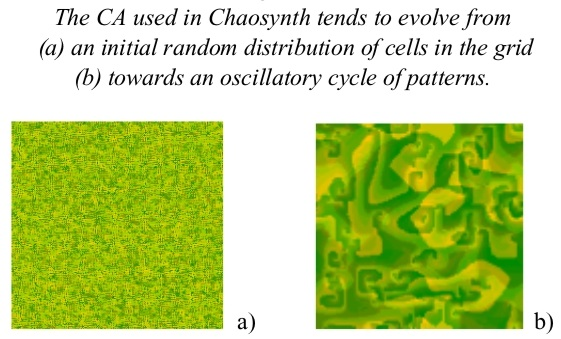
\includegraphics[scale=0.52]{chaosynth.jpg}
  \caption{Evolução de Padrões no Chaosynth~\cite{miranda2003music}}
  \label{fig:chaos1}
\end{figure}

Os estados possíveis são quiescente, despolarisado ou queimado, e se relacionam
com valores de "corrente elétrica". Esses valores dependem do estado anterior 
de determinada célula, bem como do estado de seus vizinhos. Basicamente, uma 
célula quiescente começa a se despolarizar, e ao atingir um limite de 
despolarização, dispara e queima. Uma celula queimada num instante \textit{t} 
é substituída por uma quiescente no instante \textit{t + 1}.

Uma distribuição aleatória de células na grade do Chaosynth tende a um ciclo de
padrões oscilatórios, e a soma dos sons produzidos pelos grânulos representados
nas células forma eventos sonoros maiores.

O material produzido nas iterações do Game of Life e do Chaosynth é utilizado 
nos passos seguintes do CAMUS, e o resultado é um material musical utilizado 
nas composições dos autores. Exemplos de composições utilizando 
material desses sistemas são 
\textit{Entre l'absurde et le mystere - for chamber orchestra}, 
\textit{Wee Batucada Scotica} e \textit{Olivine Trees}.

\subsubsection{An Artificially Intelligent Jazz Performer}

Neste artigo~\cite{ramalho99} é apresentado um Sistema Musical Multiagente que 
um consiste em um modelo para simulação de um baixista de uma banda de Jazz, 
que interage com outros músicos durante uma performance ao vivo.

\begin{figure}[H]
  \centering
  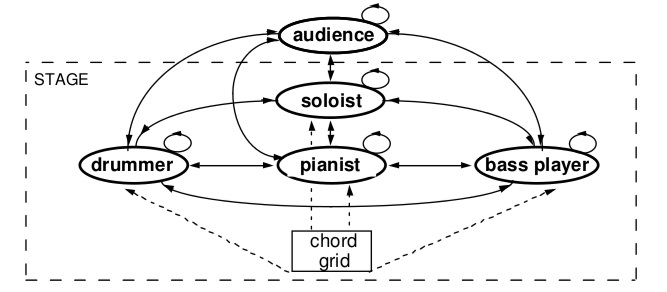
\includegraphics[scale=0.44]{jazz.jpg}
  \caption{Mapa de Interações do Agente Musical~\cite{ramalho99}}
  \label{fig:mapa}
\end{figure}

Na performace de Jazz, existe uma grande diferença entre as instruções da 
partitura e o que está sendo tocado pelos músicos. Para lidar com esta 
diferença, o Agente Musical deve armazenar fragmentos melódicos previamente 
conhecidos ou escutados em sua mémoria musical, e deve também ter implementadas
em seu raciocínio regras para o uso desses fragmentos no contexto musical 
mutável da performance~\cite{ramalho99}.

\subsubsection{Living Melodies}

É um Sistema Musical Multiagente com características emergentes. Os agentes têm
comportamentos codificados em instruções, que podem se modificar ao longo da 
execução do programa, dado o contato com outros agentes e com o 
ambiente~\cite{d01living}.

Assim como no CAMUS e Chaosynth, os organismos virtuais são representados em 
uma grade, onde cada célula contém um organismo. Mas neste Sistema os 
organismos simulados são muito mais complexos, pois têm codificado em sua Base 
de Conhecimentos uma série de instruções comportamentais que podem ser mutadas 
e transmitidas a novos organismos, no processo de reprodução. Esses Agentes 
podem se mover pelo Ambiente, escutar som produzido por
outros Agentes e interagir com eles.

\begin{figure}[H]
  \centering
  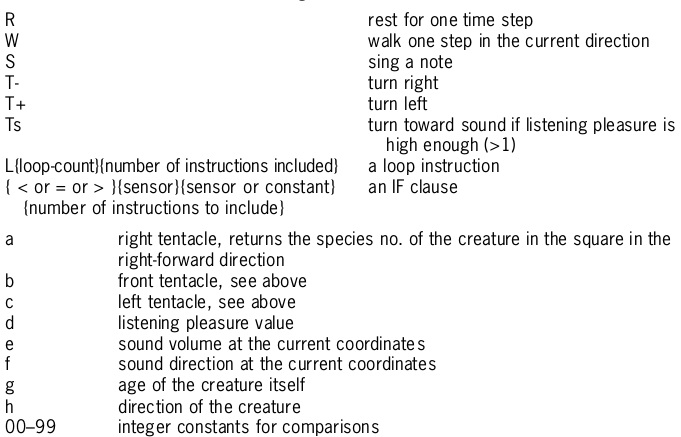
\includegraphics[scale=0.44]{table12.jpg}
  \caption{Instruções e Parâmetros Constituintes do Genoma~\cite{d01living}}
  \label{fig:livingmel1}
\end{figure}

O comportamento das diferentes espécies de Agente definidas no Living Melodies 
é determinado por seu genoma procedural e sonoro. O genoma procedural define 
uma sequência de ações a ser realizada pelo Agente e também seu mecanismo de 
produção sonora, e o genoma sonoro contém as notas musicais favoritas desse 
Agente.

\begin{figure}[H]
  \centering
  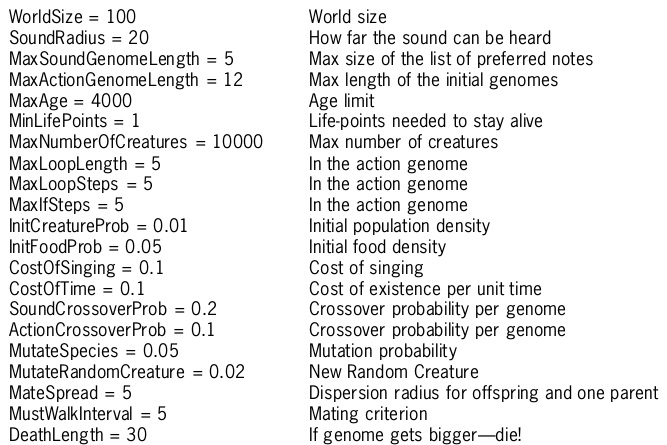
\includegraphics[scale=0.44]{table4.jpg}
  \caption{Parâmetros da Simulação~\cite{d01living}}
  \label{fig:livingmel2}
\end{figure}

Os Agentes podem se reproduzir desde que atinjam alguns criterios definidos 
na implementação, como quantidade de energia, quantidade de felicidade - 
obtida ao se ouvir notas preferidas, idade e proximidade de outro Agente.

Há uma implementação do Living Melodies utilizando o Arcabouço Ensemble, e um 
passo da execução é mostrado na Figura \ref{fig:livingensemble}.

\begin{figure}[H]
  \centering
  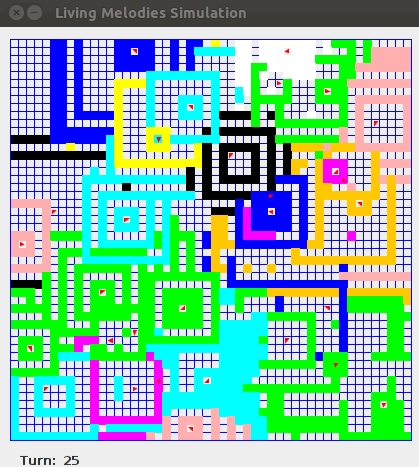
\includegraphics[scale=0.44]{livingmel.jpg}
  \caption{Living Melodies no Ensemble~\cite{leandro11}}
  \label{fig:livingensemble}
\end{figure}

O som produzido pelo Living Melodies dependerá do que for emitido pelos 
Agentes contidos na simulação, além da quantidade de felicidade dos Agentes 
emissores e de outros parâmetros definidos, como por exemplo
a localização do ouvinte no Ambiente virtual.

\subsubsection{Projeto Andante}

O Projeto Andante consiste em uma infraestrutura de código aberto para a 
construção de aplicações distribuídas para composição e performance musical 
baseadas em agentes móveis musicais~\cite{ueda2003andante}.

Um Agente capaz de se migrar entre máquinas conectadas por uma rede é chamado 
Agente Móvel. Este tipo de Agente tem autonomia, dentro do Sistema, para 
decidir o que fazer na máquina em que se encontra e quando migrar para outra 
máquina.

O conceito de Agente Móvel surgiu na década de 90~\cite{johansen1995operating},
apresentando um novo paradigma para sistemas computacionais distribuídos e 
móveis.

\section{Ensemble}

O Ensemble é um arcabouço para a construção de Sistemas Musicais Multiagentes, 
desenvolvido e descrito por Thomaz~\cite{leandro11} e 
Santiago~\cite{santiago12}, e tem como público alvo a comunidade de músicos que
utiliza o computador como ferramenta de criação musical, fornecendo os serviços
e ferramentas necessários para a criação de Sistemas Musicais Multiagentes. 

O arcabouço contém uma série de classes que permitem fácil extensão pelo
código cliente, além de um complexo sistema interno para
controle temporal e de execução.

A programação de novos componentes para o Ensemble requer conhecimento de seu 
funcionamento, e deve seguir as convenções de programação do arcabouço. 

\subsection{Arquitetura}

A arquitetura~\cite{leandro11} do Ensemble segue o paradigma de programação 
orientada a objetos, exigindo uma linguagem capaz de implementá-lo.

A presente implementação do Ensemble foi codificada em linguagem Java, a fim de
permitir que aplicações musicais possam ser executadas em plataformas 
distintas.

A arquitetura utiliza o middleware para sistemas multiagentes 
JADE~\cite{belli99}, que provê a infraestrutura necessária para manter o ciclo 
de vida dos Agentes e controlar a troca de mensagens entre eles.

São utilizadas principalmente três funcionalidades do JADE na implementação do
Ensemble, o serviço de agendamento de tarefas, o mecanismo de troca de mensagem
entre os agentes e o serviço de diretório.

\subsubsection{Arquitetura de Aplicação}

Uma aplicação do Ensemble deve estender e utilizar um conjunto de classes
específicas, dependente das funcionalidades desejadas. Apesar disso,
toda aplicação deve ser composta de alguns componentes-chave. 

É necessário definir um Agente Ambiente e um Mundo, que serão as classes
utilizadas pelo Ensemble para controlar a execução da aplicação,
e fornecerão um ambiente virtual específico para os Agentes Musicais.

A aplicação pode então adicionar Agentes Musicais e seus componentes, 
como Raciocínios, Bases de Conhecimento, Atuadores e Sensores, e esses
componentes também terão sua execução controlada pelo Ensemble, pois
estarão vinculados a um Agente Ambiente.

\begin{figure}[H]
  \centering
  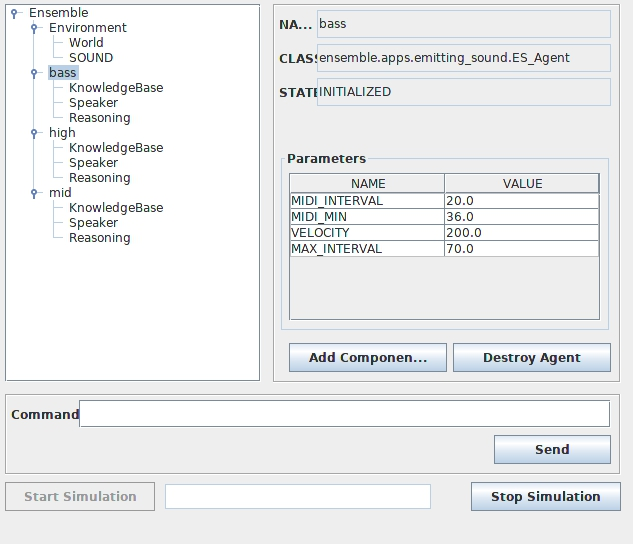
\includegraphics[scale=0.35]{ensemble_sniffer_ext.jpg}
  \caption{Exemplo de Extensão do Ensemble}
  \label{fig:sniffer}
\end{figure}

A Figura \ref{fig:sniffer} demonstra, através do Sniffer, a arquitetura 
de uma extensão simples
do arcabouço, que conta com três Agentes emissores de notas
MIDI no Ambiente Virtual. Note a Base de Conhecimentos, 
o Raciocínio e um Atuador cadastrados
para cada Agente Musical. Ainda é possível observar os
parâmetros contidos na Base de Conhecimentos de cada
Agente, referentes às características do som que eles emitem.

O usuário deve escolher a interface de áudio que vai utilizar,
e definir os tipos de eventos que serão tratados por sua aplicação.
Isso é feito através da extensão das classes de Servidores de Eventos.
As classes de Atuadores e Sensores definirão o tratamento dos tipos
de eventos cadastrados pelos Servidores de Evento.

\subsection{Interfaces}

O Ensemble é capaz de interagir com sistemas externos, usuários ou 
bibliotecas de processamento de áudio, e tem suporte a vários protocolos de 
comunicação. Essas interfaces permitem incorporar recursos de processamento 
sonoro ou ferramentas para criação e gerenciamento de Agentes, que provêm de 
outras bibliotecas e enriquecem as funcionalidades do arcabouço.

Uma interface gráfica, baseada no Agente \textit{Sniffer} disponível no 
middleware JADE~\cite{belli99}, permite o controle e monitoramento visual do 
sistema.

Essa interface permite o envio de mensagens customizadas para um determinado 
componente do sistema, a criação e destruição de Agentes musicais, e a inserção
e remoção de componentes e Ambientes. Além disso, é possível visualizar todos 
os Agentes, componentes registrados e seus estados internos, e alterar qualquer
um de seus parâmetros~\cite{leandro11}.

O arcabouço Ensemble é capaz de se comunicar via protocolo Open Sound 
Control, podendo receber mensagens enviadas por \textit{patches}
Pure Data e enviar suas próprias mensagens~\cite{leandro11}. 

Essa comunicação permite a um \textit{patch} Pd ter acesso a estados e 
parâmetros do Ambiente Ensemble e de Agentes no arcabouço.

O protocolo de comunicação Open Sound Control é uma sintaxe que permite troca 
de mensagens entre computadores, sintetizadores e softwares, possui um sistema 
de nomenclatura capaz de endereçamento de mensagens a múltiplos destinatários, 
mecanismos de pacotes de mensagens (\textit{bundles}) e controles 
temporais de alta resolução (\textit{time tags})~\cite{wright97}.

O Ensemble tem incorporadas duas bibliotecas Java para processamento digital de
sinais, a aubio~\cite{aubio01} e a LibXtract~\cite{libx01}.

Para interfaces de entrada/saída de áudio, podem ser utilizados o 
JACK~\cite{jack01}, o PortAudio~\cite{port01} e o JavaSound~\cite{jsnd01}, 
todos através da JNI (Java Native Interface)~\cite{JNI}.

É possível incorporar novas bibliotecas de processamento sonoro ou de 
entrada/saída de áudio através de código Java, caso essas bibliotecas
tenham sido implementadas nessa linguagem, ou através de código nativo
com a JNI.

\section{Pure Data}

A linguagem de programação visual Pure Data, ou \textbf{Pd}~\cite{puckette97}, 
é uma ferramenta tradicionalmente utilizada por músicos no processo de criação
e composição de material musical~\cite{leandro11}. 

A entrada de um programa em Pure Data é tratada como
um fluxo de informação, que é direcionado e processado
em blocos, produzindo uma saída em tempo real.

A linguagem fornece abstrações de alto nível que encapsulam
diversas funcionalidades, como operações matemáticas,
de entrada/saída, e outras operações sobre sinais.

Um programa é composto pela conexão dessas
funcionalidades, ou objetos, e é chamado de \textit{patch}.

\begin{table}[H]
    \centering
    \begin{tabular}{|l|}\hline
        Pure Data\\[0.07in]
        \begin{tabular}{|l|}\hline
            Interface Gráfica\\\hline
            \\
            Múltiplos Patches;\\
            Threading;\\
            Controle Temporal;\\
            Processamento de Sinais;\\
            \\
            \hline
            API de Áudio\\[0.07in]
            \hline
        \end{tabular}
        \\
        \\
        \hline
    \end{tabular}    
    \caption{Estrutura do Pure Data - Execução Independente.}
    \label{tab:pdstructure}
\end{table}

Trabalhando com entradas (\textit{inlets}) e saídas (\textit{outlets}) ligadas 
entre si através de \textit{patches}, é possível estruturar blocos de 
processamento e gerenciar fluxos de áudio ao longo do tempo.

O Pure Data fornece um ambiente de desenvolvimento
capaz de execução independente, e ferramentas potentes
voltadas a aplicações sonoras e musicais, porém essas 
características estão amarradas a interfaces de usuário 
e APIs de áudio que são direcionadas a certos formatos de aplicação.

A Tabela \ref{tab:pdstructure} ilustra a estrutura de uma instância do Pure 
Data enquanto executa e edita \textit{patches}. Além da interface
gráfica e da saída de áudio, é possível trocar informação com um patch através
de mensagens OSC, entrada/saída de amostras e mensagens de 
outro \textit{patch}.

\subsection{libpd}

A libpd é uma biblioteca de funções que permite utilizar patches e 
funcionalidades do Pure Data no contexto de outras aplicações,
encapsulando e simplificando a interface do Pure Data com o
desenvolvedor e com outras linguagens de programação~\cite{libpd1}.

Uma aplicação que utiliza a libpd deve se preocupar com a inicialização do Pd
e de suas funções para callback, e com a chamada dos métodos 
de processamento nos momentos em que precisar de amostras de áudio.

Ao encapsular a interface do Pure Data, a libpd
permite a utilização de funções nativas, patches e funções de 
bibliotecas externas do Pure Data no contexto de aplicações em 
diferentes linguagens e plataformas.

Nesse processo, são removidas algumas das características
que dão independência à execução do Pd, e torna-se 
mais fácil utilizar \textit{patches} no contexto de outras aplicações.

Um \textit{patch} pode ser utilizado como um gerador de áudio,
que modifica sua saída de acordo com entradas fornecidas pela
aplicação que executa o \textit{patch}, produzindo amostras 
dependentes do contexto dessa aplicação, e que serão utilizadas 
por ela quando necessário.

Outro exemplo de utilização de \textit{patches} é o processamento de
amostras de áudio produzidas pela aplicação, e neste caso é possível
pensar no \textit{patch} como uma biblioteca de Processamento Digital
de Sinais, que pode receber amostras de áudio e sinais de controle e produzir
amostras processadas, que serão utilizadas pela aplicação.

Um \textit{patch} pode ainda ser utilizado de forma estática, como 
mecanismo de controle e configuração da aplicação, enviando mensagens
sem necessariamente processar ou produzir áudio.

A Tabela \ref{tab:libpdstructure} ilustra o encapsulamento do Pure Data através
dos métodos e abstrações implementados pela libpd. O código cliente
mantém controle sobre sua execução, e comanda os ciclos de 
processamento do Pd, definindo a taxa de amostragem, tamanho
de bloco, e quantos blocos serão recebidos por ciclo de processamento.

\begin{table}[H]
    \centering
    \begin{tabular}{|l|}\hline
        Código Cliente\\[0.07in]
        \begin{tabular}{|l|}\hline
            GUI do Código Cliente\\\hline
            \\
            Código de Alto Nível;\\
            Threading;\\
            Controle Temporal;\\
            \\
            \begin{tabular}{|l|}\hline
                libpd\\[0.07in]
                \begin{tabular}{|l|}\hline
                    Pure Data\\\hline
                    \\
                    Múltiplos Patches;\\
                    Processamento de Sinais;\\
                    \\
                    \hline
                \end{tabular}
                \\
                \\
                \hline
            \end{tabular}
            \\
            \\
            \hline
            API de Áudio do Código Cliente\\[0.07in]
            \hline
        \end{tabular}
        \\
        \\
        \hline
    \end{tabular}
        \caption{Estrutura de Código Cliente encapsulo o Pd com a libpd.}
        \label{tab:libpdstructure}
\end{table}

O código cliente pode então tratar um patch como
uma "caixa-preta" que recebe e devolve amostras
e dados, desde que o patch respeite convenções
de símbolos \textit{send} e \textit{receive}.

\section{O Protocolo}

Através da implementação da libpd na linguagem Java é possível
realizar a comunicação entre Raciocínios de Agentes inseridos no
Ensemble e \textit{patches} Pure Data. Neste contexto, o Raciocínio
Java serve como encapsulador do \textit{patch}, que contém o Raciocínio em si.

Para que este encapsulamento funcione, a implementação de um \textit{patch} 
para uma aplicação do Ensemble deve seguir um protocolo, usando objetos e
sintaxe bem definidos, para que possa acessar as estruturas contidas nas
representações de Agentes e demais componentes de uma aplicação no Ensemble.
Esse protocolo deve definir objetos Pd para acessar e modificar Memórias
correspondentes a Sensores e Atuadores, e informações na Base de Conhecimentos
de um Agente, pois essas são estruturas e informações essenciais na elaboração
de qualquer Raciocínio. Além disso, o protocolo deve definir objetos para
criação e modificação de Agentes e seus componentes, e dos Ambientes Virtuais
para execução da aplicação. Finalmente, o protocolo deve fornecer acesso às 
configurações disponíveis no arquivo XML de configuração e inicialização.

O protocolo definido a seguir procura permitir que aplicações Ensemble sejam
configuradas sem a necessidade de conhecimento da implementação do Arcabouço
em Java. Idealmente, não deve ser necessário que o usuário do Ensemble-Pd
tome conhecimento da troca de informações e mensagens entre seu \textit{patch}
Pd e o código Java do Ensemble.

\subsection{Ambiente}

Aplicações do Ensemble podem ser configuradas através de um arquivo XML
processado por uma classe de inicialização, onde o usuário define os
componentes e parâmetros de sua aplicação, como Servidores de Eventos,
Mundos e Leis, Agente Musicais e seus Componentes. A interface Ensemble-Pd
permite que esses parâmetros sejam definidos através dos argumentos de 
mensagens enviadas a símbolos no Pd no momento de inicialização do 
\textit{patch} pela instância do Pd executada no Ensemble.

Mensagens enviadas ao símbolo \textbf{global} definem o modo de
execução do relógio interno, processamento e agendamento do Ensemble;
mensagens enviadas ao símbolo \textbf{environment} definem o Agente Ambiente,
Mundo e Leis; e mensagens enviadas ao símbolo \textbf{add\_agent} definem os
nomes dos Agentes que devem ser adicionados à aplicação, cuja definição deve
estar em \textit{subpatches} ou abstrações dentro do patch de configuração.

A Tabela \ref{tab:startupsymbols} apresenta os objetos Pd utilizados no momento
da inicialização, seu uso e parâmetros.

\end{multicols}

\begin{table}[h]
    \begin{center}
        \begin{tabular}{|l|l|l|}
            \hline
            Símbolo/Objeto & Argumentos & Uso \\
            \hline
        \textbf{global} & \begin{tabular}[c]{@{}l@{}}<clock\_mode>\\<process\_mode>\\<scheduler\_threads>\end{tabular} & \begin{tabular}[c]{@{}l@{}}Define\\parâmetros\\de execução\end{tabular} \\
            \hline   
        \textbf{environment} & \begin{tabular}[c]{@{}l@{}}<class>\\<world>\\<\textit{world\_class}>\\ {[}<\textit{world\_law}>]\end{tabular} & \begin{tabular}[c]{@{}l@{}}Define\\parâmetros\\de Ambiente\\e Mundo\end{tabular} \\
            \hline
        \textbf{add\_agent} & <name> & \begin{tabular}[c]{@{}l@{}}Adiciona\\um Agente\end{tabular}\\
            \hline
        \textbf{[r <\textit{agent}>/start]} & & \begin{tabular}[c]{@{}l@{}}Recebe\\bang de\\inicialização\end{tabular} \\
            \hline   
        \end{tabular}
    \end{center}
    \caption{Símbolos de Inicialização.}
    \label{tab:startupsymbols}
\end{table}

\begin{multicols}{2}

\subsection{Sensores e Atuadores}

Todos os Agentes adicionados a uma aplicação no Ensemble-Pd têm seu próprio
\textit{subpatch} onde são definidos e configurados seu Raciocínio, 
Sensores, Atuadores, Memórias e Base de Conhecimentos. Essas mensagens
de configuração são enviadas ao Ensemble quando o Arcabouço inicializa
os Agentes.

A Tabela \ref{tab:actuatorsandsensors} mostra os símbolos e objetos
Pd utilizados na comunicação e configuração dos Sensores e Atuadores de
um Agente.

\end{multicols}

\begin{table}[H]
    \begin{center}
        \begin{tabular}{|l|l|l|}
            \hline
            Símbolo/Objeto & Argumentos & Uso \\
            \hline
        \textbf{add\_actuator} & \begin{tabular}[c]{@{}l@{}}<name>\\<type>\\ {[}<scope>]\end{tabular} & Adiciona novo Atuador \\
            \hline   
        \textbf{add\_sensor} & \begin{tabular}[c]{@{}l@{}}<name>\\<type>\\ {[}<scope>]\end{tabular} & Adiciona novo Sensor \\
            \hline
            \textbf{remove\_actuator} & <name> & Remove um Atuador \\
            \hline
            \textbf{remove\_sensor} & <name> & Remove um Sensor \\
            \hline
        \textbf{[s \textit{actuator\_name}]} & \begin{tabular}[c]{@{}l@{}}<data>\\ {[}<scope>]\end{tabular} & \begin{tabular}[c]{@{}l@{}}Escreve dados\\ em \textit{actuator\_name}\end{tabular} \\
            \hline
        \textbf{[r \textit{sensor\_name}]} & & \begin{tabular}[c]{@{}l@{}}Recebe dados\\de \textit{sensor\_name}\end{tabular} \\
            \hline
        \end{tabular}
    \end{center}
    \caption{Símbolos para Atuadores e Sensores.}
    \label{tab:actuatorsandsensors}
\end{table}

\begin{multicols}{2}

O Ensemble inicializa o processamento dos Agentes enviando, através da libpd,
um \textbf{bang} para o símbolo \texttt{<\textit{agent}>/start} 
(veja a Tabela \ref{tab:startupsymbols}), que será recebido no \textit{patch}
através do objeto \pdobject{r <\textit{agent}>/start} ao qual devem estar
conectadas as mensagens de inicialização do Agente.

\subsection{Base de Conhecimentos}

Mensagens enviadas ao símbolo \textbf{new\_fact} adicionam um novo Fato
à Base de Conhecimentos de um Agente, e devem conter um nome e um valor.
Fatos adicionados podem ser recuperados e modificados através dos objetos
Pd \pdobject{read\_fact <agent\_name>} \pdobject{update\_fact <agent\_name>} 

Na Tabela \ref{tab:kbprotocol} estão os símbolos e objetos utilizados no
acesso e modificação da Base de Conhecimentos de um Agente.

\end{multicols}

\begin{table}[H]
    \begin{center}
        \begin{tabular}{|l|l|l|}
            \hline
            Símbolo/Objeto & Argumentos & Uso \\
            \hline
        \textbf{new\_fact} & \begin{tabular}[c]{@{}l@{}}<agent>\\<name>\\<value>\end{tabular} & Adiciona novo Fato\\
            \hline   
        \textbf{update\_fact} & \begin{tabular}[c]{@{}l@{}}<agent>\\<name>\\<value>\end{tabular} & \begin{tabular}[c]{@{}l@{}}Atualiza um\\fato se ele\\existir\end{tabular}\\
            \hline
            \textbf{remove\_fact} & name & Remove um Fato\\
            \hline
        \textbf{[read\_fact]} & \begin{tabular}[c]{@{}l@{}}<agent>\\<name>\\<value>\end{tabular}
                              & \begin{tabular}[c]{@{}l@{}}Lê um \\Fato e\\devolve seu valor\end{tabular}\\
            \hline
        \end{tabular}
    \end{center}
    \caption{Símbolos para a Base de Conhecimentos.}
    \label{tab:kbprotocol}
\end{table}

\begin{multicols}{2}

\subsection{Memórias}

Da mesma forma, diferentes tipos de Memórias podem ser criadas, acessadas e
modificadas através de mensagens aos símbolos \textbf{new\_memory}, 
\textbf{read\_memory} e \textbf{write\_memory}. 

A Tabela \ref{tab:memprotocol} contém os símbolos e objetos utilizados
pelo protocolo na manipulação de Memórias.

\end{multicols}

\begin{table}[H]
    \begin{center}
        \begin{tabular}{|l|l|l|}
            \hline
            Símbolo/Objeto & Argumentos & Uso \\
            \hline
        \textbf{new\_memory} & \begin{tabular}[c]{@{}l@{}}<agent>\\<name>\\<type>\\\end{tabular} & Adiciona nova Memória \\
            \hline 
        \textbf{write\_memory} & \begin{tabular}[c]{@{}l@{}}<agent>\\<name>\\<value>\end{tabular} & \begin{tabular}[c]{@{}l@{}}Escreve numa \\Memória no\\instante atual\end{tabular} \\
            \hline
        \textbf{read\_memory} & \begin{tabular}[c]{@{}l@{}}<agent>\\<name>\\<time>\end{tabular} & \begin{tabular}[c]{@{}l@{}}Lê uma \\Memória e\\devolve um valor\end{tabular} \\
            \hline
        \end{tabular}
    \end{center}
    \caption{Símbolos para Memória.}
    \label{tab:memprotocol}
\end{table}

\begin{multicols}{2}

\section{A Interface}

A interface implementada é composta de uma extensão do Arcabouço Ensemble,
que consiste de várias classes Java e de algumas abstrações Pure Data.
Esta seção descreve com detalhes a implementação das classes e abstrações,
e discute os problemas encontrados e as soluções adotadas.

\subsection{Classes Java}

Esta seção apresenta uma descrição detalhada da interface Ensemble-Pd,
justificando as principais classes Java utilizadas, expondo suas 
interrelações e contextualizando seu papel no funcionamento de aplicações
do Ensemble.

\subsubsection{PdAgent}

Esta classe é uma extensão da classe \textbf{MusicalAgent} do Ensemble,
e suas instâncias representam agentes musicais numa aplicação.
O mapeamento de um agente definido num \textit{patch} e sua representação no 
Ensemble é feito através dessa classe.

A classe \textbf{PdAgentClassInformation} encapsula informações sobre
instâncias de Agentes definidas no \textit{patch}, que são utilizadas na
inicialização do Ensemble para instanciar e cadastrar esses Agentes no
JADE.

Os componentes de um Agente, como Raciocínio, Atuadores e Sensores, são
adicionados a \textbf{PdAgent} através de mensagens definidas dentro do
\textit{patch}. Atuadores e Sensores são representados pelas classes 
\textbf{PdActuator} e \textbf{PdSensor}, respectivamente.

O Servidor de Eventos de uma aplicação Ensemble-Pd é responsável por garantir 
que a representação de um Agente num \textit{patch} receba e envie Eventos, 
Mensagens e Áudio de e para o Ambiente Virtual e outros Agentes. Isso é feito
através de Sensores e Atuadores especiais, inseridos por padrão em instâncias
de \textbf{PdAgent}, e que permitem essa comunicação.

\subsubsection{PdReasoning}

O raciocínio de um Agente numa aplicação Ensemble-Pd é definido dentro do
\textit{subpatch}/abstração correspondente a esse Agente, e consiste de
uma aplicação Pd que pode conter qualquer objeto Pd utilizado em aplicações
tradicionais. De dentro do \textit{patch} de Raciocínio, o programador Pd tem 
acesso à informação recebida pelo Agente através dos Sensores que ele definiu,
podendo utilizar os recursos de Processamento de Sinais implementados no Pure
Data para produzir e processar amostras de áudio e demais informações 
recebidas, e pode atuar no Ambiente Virtual através dos Atuadores do Agente.

\subsubsection{PdEvent}

Esta classe encapsula, no funcionamento de uma aplicação Ensemble,
as mensagens e informações provenientes e destinadas a \textit{patches} Pd.

Os tipos manipulados por esta classe são \textbf{PdFloat}, \textbf{PdMessage} e
\textbf{PdAudioBlock}, que por sua vez encapsulam os diferentes tipos de dados
tratados pelo Pure Data.

\subsubsection{PdServer}

Esta é a principal classe do ponto de vista da sincronização 
e mapeamento entre \textit{patches} e aplicações Ensemble.
Ela é quem centraliza e coordena a execução de um \textit{patch}, utilizando
a classe \textbf{PdProcessor}, e processa as mensagens e dados recebidos do Pd 
através da classe \textbf{PdReceiver}, produzindo Eventos para os Sensores 
dos Agentes a que essas mensagens se destinam.

Além disso, é ela quem processa os Eventos enviados por Atuadores de Agentes,
reproduzindo no \textit{patch} as mudanças feitas pelos Agentes.

\subsubsection{PdReceiver}

Esta é uma extensão da classe \textbf{PdDispatcher} contida na implementação
Java da libpd, e encapsula as funções de \textit{callback} usadas na
comunicação entre \textit{patches} e aplicações que usam a libpd.

Esta classe também é responsável por registrar e gerenciar símbolos
usados na comunicação do Ensemble com o \textit{patch}, centralizando
o envio e recebimento de mensagens, áudio e demais informações.

A padronização dos símbolos utilizados nos componentes e mensagens
de uma aplicação Ensemble-Pd permite que o ciclo de processamento
dos \textit{patches} de aplicação seja centralizado pela classe
\textbf{PdServer}, pois garante que não haverão ambiguidades entre
destinatários/remetentes e que nenhuma mensagem será perdida
entre ciclos de processamento.

\subsubsection{PdAudioBlock}

Durante a implementação da interface, desenvolvemos duas diferentes estratégias
para a transferência de amostras de áudio entre o \textit{patch} e o Ensemble, 
uma centralizada e uma distribuída, finalmente optando pela centralização 
do ciclo de processamento na classe \textbf{PdServer}.

A estratégia distribuída consistia na descentralização dos ciclos de
processamento da libpd, permitindo que cada Raciocínio de um Agente
inserido numa aplicação processasse seu \textit{subpatch} independentemente,
tratando suas próprias mensagens e amostras de áudio separadamente.

Essa estratégia gera problemas de sincronização de Eventos e Áudio,
decorrentes do funcionamento dos dois softwares envolvidos.

As amostras de áudio produzidas num mesmo momento pelos Agentes 
num \textit{patch} devem ser tocadas como seriam num \textit{patch}
processado pelo Pd, e as mensagens enviadas pelos Agentes devem obedecer
uma sequência definida pelo Raciocínio, também definido num \textit{patch}.
Se cada Agente é capaz de processar o \textit{patch} de aplicação
no seu ciclo de processamento no Ensemble, não é possível garantir que ele
não receberá ou enviará Eventos ou Áudio somente após todos os outros Agentes 
recebam seu "turno" de Eventos, pois o controle de tempo execução dos Agentes 
é feito pelo middleware JADE, e não tem conexão com o ciclo de processamento
da libpd.

Como o \textit{patch} de configuração de aplicação é único, o controle de
processamento descentralizado produz desencontros nas amostras de Áudio, 
e também no fluxo de Eventos da aplicação.

A solução de processamento centralizado resolve estes problemas utilizando
as abstrações Pd \textbf{act\textasciitilde} e \textbf{sense\textasciitilde},
e as classes Java \textbf{PdAudioBlock} e \textbf{PdAudioBlockStream}.

Essas classes representam um bloco de processamento do Pure Data, e um
encadeamento temporal desses blocos, respectivamente. Elas permitem
receber amostras de Áudio de cada Atuador independentemente, e enviar
amostras a Sensores de forma sincronizada, pois cada Sensor e Atuador
tem seu próprio \textbf{PdAudioBlockStream}.

O Servidor de Eventos pode então enviar e receber Áudio e Eventos de Agentes,
mantendo a sincronia entre a execução do Ensemble e o processamento 
do \textit{patch}.

\subsection{Abstrações no Pure Data}

Em conjunto com as classes Java foram implementadas abstrações do
Pure Data, que são facilitadores da comunicação entre Ensemble e Pd
e encapsulam o uso dos componentes de baixo-nível fornecidos pela
interface Ensemble-libpd em  novos componentes de alto-nível
na forma de objetos Pure Data.

O programador Pd pode então utilizar esses objetos para se comunicar
com o Ensemble utilizando as convenções da linguagem Pure Data,
sem se preocupar com detalhes de implementação da interface com o
Ensemble.

\subsubsection{act\textasciitilde e sense\textasciitilde}

Um Atuador de um Agente numa aplicação é representado pela abstração
\textbf{act\textasciitilde}, e recebe através de um \textit{inlet} 
um sinal de Áudio que será propagado no Ambiente 
Virtual e percebido por outros Agentes de acordo com as regras da aplicação. 
De forma análoga, a abstração \textbf{sense\textasciitilde} possui um 
\textit{outlet} através do qual o \textit{patch} recebe os sinais de Áudio 
percebidos pelo Agente correspondente.

As abstrações \textbf{act} e \textbf{sense}, seguindo a convenção de nomes do
Pure Data, são utilizadas para a comunicação dos demais tipos de dados.

\subsubsection{read\_memory\textasciitilde e read\_fact}

Estas abstrações são utilizadas para acessar informações da Base
de Conhecimentos ou da Memória de Agentes numa aplicação. O objeto
\textbf{read\_memory\textasciitilde} é usado para ler a Memória de
sinais de Áudio de um Atuador ou Sensor de um Agente, e possui
um \textit{outlet} através do qual o \textit{patch} recebe o sinal
de Áudio correspondente ao Componente e intervalo temporal determinados
na inicialização do objeto.

O objeto \textbf{read\_fact} lê da Base de Conhecimentos de um Agente
o Fato cujo nome de identificação é definido em sua inicialização, ou
através de mensagens. O \textit{patch} acessa esse Fato através do
\textit{outlet} deste objeto.

\subsection{Código e Documentação}

O código e a documentação do Arcabouço Ensemble podem ser encontrados
respectivamente em~\cite{ensemblecode} e~\cite{ensembledoc}.
O projeto tem uma página~\cite{ensemblegrouppage} no site do Grupo de Computação 
Musical do IME, e o código pode ser obtido seguindo as instruções na própria página
onde está hospedado.

\section{Disciplinas Cursadas}

Durante este último semestre, foram cursadas três disciplinas no IME.
Esta seção fará um breve comentário sobre cada uma delas.

\subsection{Conceitos Fundamentais de Linguagens de Programação}

Nesta disciplina foi construída uma linguagem de programação muito
simples, sobre a linguagem \textit{Racket}. No processo, estudou-se
as estruturas sintáticas e semânticas necessárias para a elaboração
de uma linguagem de programação, por meio da implementação dessas
estruturas. A linguagem no estado final contém, por exemplo,
implementações de Funções, Objetos, Ambientes e Escopos.

\subsection{Laboratório de Programação Extrema}

Aborda metodologias de desenvolvimento de software, e as
diversas técnicas e ferramentas aprendidas são exercitadas em
um projeto real. Contribuiu para o Projeto de Iniciação Científica
do aluno com noções de planejamento, organização e integração contínua
no processo de desenvolvimento de software.

\subsection{Princípios de Interação Humano-Computador}

Esta disciplina estuda o planejamento de interfaces de software voltadas 
ao usuário, os conceitos e ferramentas abordados também são exercitados
em um projeto de desenvolvimento de interface. Esta disciplina contribui com
os objetivos do Projeto de Iniciação Científica desenvolvido pelo aluno,
pois abordou princípios de elaboração de interfaces e de design centrado
no usuário.

\section{Conclusão}

Os objetivos do Projeto foram atingidos, pois o protocolo definido mapeia
os conceitos e funcionalidades do Arcabouço Ensemble em abstrações,
mensagens e símbolos de um \textit{patch} Pure Data, e a interface Ensemble-Pd
permite a implementação de Agentes, Ambientes e Raciocínios do Ensemble através
do Pure Data. O protocolo e a interface permitem a um usuário implementar 
aplicações do Arcabouço Ensemble mesmo que ele não possua conhecimento sobre
programação em linguagem Java, desde que saiba programar em Pure Data. 
No entanto, algumas flexibilidades características do Arcabouço são perdidas
devido ao alto nível de abstração da interface do Pure Data, sendo ainda 
necessário o conhecimento de Java para implementar, por exemplo, novas leis 
de propagação sonora ou de interação entre os Agentes, e novos tipos de dados
a ser tratados pela Aplicação, como por exemplo novos tipos deEventos do 
Ensemble.

\end{multicols}

\newpage
\bibliographystyle{plain}
\bibliography{Projeto}

\end{document}
